\documentclass[11pt,a4paper]{ltjsreport}
\usepackage{luatexja-fontspec}
\usepackage{tocloft}
\usepackage{fancyhdr} % ヘッダ・フッター用
\usepackage{makeidx} %目次表目次図目次の出力
\usepackage{lscape}
\usepackage{url} %参考文献のURL途中改行
\usepackage{tikz} %TeXで図を描きたい人用
\usepackage{amsmath} %数式用
\usepackage{titlesec} %chapterなどのタイトルフォントの大きさを調整したい時用

% \titleformat{\chapter}[display]{\huge\bfseries}{第\ \thechapter \ 章}{40pt}{}[]
%jsreportだとChapterのフォントサイズがデカくて恥ずかしいのでここで調整している

\newcommand{\bhline}{\noalign{\hrule height 1.2pt}} % 太い横線の定義(表の上部の太線用)
\renewcommand{\baselinestretch}{1.6}

%------章はじめのページにヘッダーとフッターを付けるための処理
\makeatletter
\renewcommand{\chapter}{%
    \if@openleft\cleardoublepage\else
    \if@openright\cleardoublepage\else\clearpage\fi\fi
    %\plainifnotempty %元: \thispagestyle{plain}
    \global\@topnum\z@
    \if@english \@afterindentfalse \else \@afterindenttrue \fi
    \secdef
    {\@omit@numberfalse\@chapter}%
    {\@omit@numbertrue\@schapter}}
\makeatother
%------ここまで章はじめのページにヘッダーとフッターを付けるための処理

% 目次のインデント調整
\cftsetindents{chapter}{0em}{5em} % 章
\cftsetindents{section}{2em}{3em} % 節
\cftsetindents{subsection}{4em}{3em} % 小節

\begin{document}

%------表紙
\begin{titlepage}
    \null
    \vfil
    \begin{center}
        {\huge\textbf{チャットの吹き出しにおけるアニメーション\\効果とインタラクションの研究}\par}\vskip 8em minus 2em %2行にする場合は、象の卵の\\デザイン みたいに\\をいれる
        \begin{table}[htb]
            \renewcommand{\arraystretch}{1.3}
            \centering
            \begin{tabular}
                {@{\vrule width 1.8pt\ }c|c|c@{\ \vrule width 1.8pt}}
                \noalign{\hrule height 1.8pt}
                \multicolumn{3}{@{\vrule width 1.8pt}c@{\ \vrule width 1.8pt}}{\large \   筑波大学 デザイン学学位プログラム  \ } \\
                \multicolumn{3}{@{\vrule width 1.8pt}c@{\ \vrule width 1.8pt}}{\textbf{{\Large{}}}}              \\ \hline
                \multicolumn{2}{@{\vrule width 1.8pt}c|}{\large \ 卒 業 年 度} & \large 令和6年度                        \\ \hline
                \multicolumn{2}{@{\vrule width 1.8pt}c|}{\large \ 指 導 教 員} & \large 山田博之                         \\
                \noalign{\hrule height 1.8pt}
            \end{tabular}
        \end{table}

        \par \vskip 10em
            {\Large\textbf{筑波大学 人間総合科学術院 人間総合科学研究群\\デザイン学学位プログラム 博士前期課程}}
        \vskip 2em
            {\Large\textbf{徳永 萌}\par}\vskip 2em minus 2em
        \vskip 2em
            {\Large\textbf{令和 年 月 日}}\vskip 2em minus 2em
    \end{center}
    \vfil
    \setcounter{page}{1}
\end{titlepage}
\newpage
%------ここまで表紙

%------要旨
\thispagestyle{empty}
\begin{center}
    {\Large\textbf{An Elephant Egg Design}\par}\vskip 2em minus 2em
\end{center}

\noindent
\textbf{Abstract\ }
Have you ever imagined an elephant egg?
I've created it.
Have you ever imagined an elephant egg?
I've created it.
Have you ever imagined an elephant egg?
I've created it.
Have you ever imagined an elephant egg?
I've created it.
Have you ever imagined an elephant egg?
I've created it.
Have you ever imagined an elephant egg?
I've created it.
Have you ever imagined an elephant egg?
I've created it.
Have you ever imagined an elephant egg?
I've created it.
Have you ever imagined an elephant egg?
I've created it.

\vskip 2em minus 2em

\noindent
\textbf{あらまし\ }
オンライン上でコミュニケーションをとる手段は様々であり、その代表的なツールとして
メッセージアプリによるテキストチャットやイラストなどを使用したスタンプ機能、リアクション機能などが挙げられる。
本研究ではこのような既存の機能に対しユーザー同士が相互にインタラクションすることができる機能を
搭載したツールの提案・効果の調査を行った。

非言語情報をメッセージアプリ上で伝える手段は多くはなく、

\vskip 2em minus 2em
\noindent
keyword, keyword, keyword, keyword, keyword, keyword
%------ここまで要旨

%------目次
\clearpage
\setcounter{page}{0}\pagenumbering{roman}\pagestyle{plain} %ローマ数字のページ番号セット
\setcounter{tocdepth}{2} % \subsection まで目次に表示
\tableofcontents%目次
\listoffigures%図目次
\listoftables%表目次
\clearpage
%------ここまで目次

\setcounter{page}{0}\pagenumbering{arabic} %アラビア数字のページ番号セット

%------本文のヘッダとフッタの設定
\pagestyle{fancy}
\fancyhead{} % clear all header fields
% \lhead{} %ヘッダ左
\renewcommand{\chaptermark}[1]{\lhead{第\ \thechapter\ 章~~~#1}{}}
\chead{} %ヘッダ中央
\rhead{\thepage} %ヘッダ右 ページ番号
\lfoot{} %フッタ左
\cfoot{} %フッタ中央.ページ番号を表示
% \rfoot{造形・メディアデザインコース} %フッタ右
\renewcommand{\footrulewidth}{0.5pt} %フッタの罫線
%------ここまで本文のヘッダとフッタの設定

%------本文開始
\chapter{はじめに}
\section{研究の背景}
日常生活においてテキストを用いたコミュニケーションは頻繁に行われており、
メッセージアプリ上でコミュニケーションを行うことは必要不可欠である。
X(旧Twitter)やLINEをはじめとしたSocial Networking Service(SNS)の利用者数は増加し続けている。
特にメッセージ機能をもつコミュニケーション用メッセージアプリは高い利用率となっている\cite{Web1}。
しかし、文章で多くのやり取りを行うコミュニケーション上では、会話のニュアンスをつかむことは難しく、
相手と親睦を深められたかの実感を得ることは難しい。
相互理解や相互に感情を伝えること、深め合いつつ合意形成することは非言語情報なしでは困難であり、
メールなどのテキストベースのコミュニケーションでは相手に感情や声のトーンなどの非言語情報を伝えることができないため、
対人関係のトラブルを招くことがある \cite{Thesis2}。
また、SNS上のトラブルは「SNS疲れ」を引き起こし、長時間の利用に伴う精神的・身体的疲労のほか、
自身の発言に対する反応を気にすることにより、知人の発言に返答することに義務を感じる現象が見られた\cite{Thesis2}。
その対策として、メッセージアプリ内での円滑なコミュニケーションを行うための手段であるスタンプやリアクション、
ボイスメッセージなどが挙げられる。
対面コミュニケーションにおいて得られる相手の話し方や表情、動きから読み取ることができる非言語情報は、
文字や記号、イラストを組み合わせ動きや音声を付けることで表現されている。
このように既存のサービス内のメッセージ機能には様々な非言語情報を伝える手段が存在するが、
その種類は感情を表現したイラストや、ジェスチャー、絵文字にとどまっており、
さらなる検討が必要であると考えられる。よって本研究では既存のメッセージアプリに加え非言語情報を伝達する手法を提案する。
野村らによればメッセージアプリの吹き出しの色や形を変え、
文字や吹き出しに動きをつけることは感情表現の手法として有効であることが実証されている\cite{Thesis2}。
そこで、本研究ではメッセージアプリ上で吹き出しに“触れ合う”という概念を導入し提案・評価を行う。



\section{研究の目的}
本研究の目的は、メッセージアプリにおいて非言語情報を効果的に伝える新しい手法を提案することである。
従来のテキストベースのやり取りでは伝わりにくい感情や動作を、吹き出しに触れ合うことでより自然に表現し、
コミュニケーションの質を向上させる。吹き出しを通じた触れ合いは、
お互いが同じものに触れているような感覚を生み出し、親密度を高め、相手との仲を深めることが期待される。
従来のスタンプや絵文字では伝えきれない微細な感情や、会話の中での小さな動作
(例えば、軽い突っ込みのような表現)が吹き出しを通じて効果的に伝わると考えられる。
これにより、相手からのリアクションに対してより具体的な返答が生まれ、コミュニケーションの深化が期待される。
また、ビデオ通話や通話が難しい状況下、あるいはそれを望まない場面でも、この手法を用いることで相手の存在を感じ、
コミュニケーションのぬくもりを保つことが可能であると考える。これにより、
異なる状況下での柔軟で温かいコミュニケーションが実現される。
本研究では新しいメッセージアプリの機能を通じて、ユーザーにより深いコミュニケーション経験を提供し、
感情表現の幅を拡げることを目指している。

\section{本論文の構成}
本論分は、本章を含め5章で構成されている。第2章では本研究と関連する研究について述べる。
第3章では提案ツールについて説明し、
第4章では実験内容および評価方法について述べる。第5章では結論としてまとめている。

%  卒業論文や修士論文を書くにあたって注意すべき点を挙げます。
%   \begin{itemize}
%       \item 参考文献の挙げる順序には,一貫性を持たせましょう。
%             よくある例としては以下のようなものがあります。
%       \begin{itemize}
%           \item 論文中での出現順(こちらのTeXサンプルは出現順になっています。指導教員の指示に従ってください)
%           \item 参考文献の筆者の名前順
%           \item 参考文献の出版年月順
%       \end{itemize}
%       \item 参考文献で挙げたものは,本文中で言及しなければいけません。
%       \item 参考文献番号はこんな感じでつけます
%   \end{itemize}

%  代表的なイグノーベル賞受賞研究として、栗原ら\cite{Thesis1}のSpeechJammerがある。
%  三上\cite{Book1}は「象は鼻が長い」という日本語の文法表現について論じている。
%  象の旅\cite{Book2}は、ノーベル賞作家のサラマーゴが執筆した史実に基づく作品である。
%  香川大学の造形・メディアデザインコースでは、造形学について学べる\cite{Web}。


\chapter{関連研究・事例}

\section{オンライン上のコミュニケーションにおける感情表現の事例}
本節ではオンライン上のコミュニケーションにおける感情表現の事例について述べる。

\subsection{フェイスマーク(Smiley)、絵文字}
小澤ら\cite{Thesis2}によればEmojiがUnicodeに採用された2010年以前には、文章中における感性情報の伝達には、
文字や記号を組み合わせた電子表情である「フェイスマーク(Smiley)、顔文字」が主に使われていた。
\texttt{:-)}のような「コロン」や「ハイフン」などの組み合わせで構成するSmileyは、
1970年代に欧米で文章だけでは表現しきれない感情のニュアンスを補うものとして誕生した。
これが、キーボード入力が一般的となりつつあった当時の日本の文化にも溶け込み、
フェイスマークと呼ばれて定着した。 Smileyでは: -)のように顔を転倒して表すのに対して、
フェイスマークでは\texttt{(\textasciicircum-\textasciicircum)}のように正立のまま表す場合が多い。
フェイスマークや絵文字はテキストベースのコミュニケーションツールにおいて非言語情報を伝達することが期待される一方で、
送り手の感情が正しく伝達されているという確証が得られていないのが実情である。
すなわち、多義性があり意味が曖昧なため安易に使うと誤解を生む危険性が指摘されている。

\subsection{LNEのスタンプ・リアクション機能}
LINEを主としたメッセージアプリは主に文字によってやり取りが行われるため、
対面や電話での会話と違い頷き等のジェスチャーや表情、声の調子といった非言語情報はLINE上では伝達されない。
これらの非言語情報の欠落を補完するものとしてLINEのスタンプ機能やリアクション機能が挙げられる。
スタンプ機能には、対面会話における非言語コミュニケーションの代替効果があり\cite{Thesis2}、
非言語情報の欠落を補完する役割を持つと考えられる。\cite{Thesis2}
また、リアクション機能は相手に通知されないため、スタンプ機能に比べより気軽に使用できる機能である。
LINEのような同期型のメッセージアプリでは話題の変化が激しく、
会話に対する相槌が対応するメッセージと離れて送信される場合もあるため\cite{Thesis2}、
リアクション機能は相槌のような役割も持つと考えられる。
また森本はLINE等のメッセージアプリで採択されている「スタンプ」についても感情表現やニュアンスの表現として使用されていた顔文字や絵文字と比べ、
言葉にするのが難しい生の感情を曖昧な印象として表現・伝達することを可能にし、
テキストのみのコミュニケーションであった無機質なやり取りを人間味のあるコミュニケーションに変化させたと述べている[2]。

\subsection{オンラインゲーム内でのコミュニケーション}
オンラインゲーム内で吹き出しにアイコンを付けたり吹き出しの形状を変化させる機能や(図〇)、
吹き出しの色や形を変化させ感情表現を図る研究が行われている\cite{Thesis2}。
このように吹き出しに変化を付けコミュニケーションを図る事例は存在するが、
吹き出しに触れることでコミュニケーションを図る事例は見られなかったため今回提案・調査する。

\section{メッセージアプリにおける感情伝達の手法に関する研究}
本節ではメッセージアプリにおける感情伝達に関する既存研究について述べる。

\subsection{吹き出しの色や動きについての調査}
野村ら\cite{Thesis2}はWeb上で円滑なコミュニケーションを行うための既存のメッセージアプリに付随する表現手段を抽出、
整理するとともに、それらの表現手段および表現方法と感情伝達との関係を明らかにした。
この研究ではメッセージアプリでの感情伝達の表現手段として「吹き出し」に着目し、
色や動きを変えることで感情の有効な表現手段を調査した。「吹き出し・文字の動き」、
「吹き出し・文字の動きの周期」、「吹き出しの形状」、「吹き出しの色」の4種類を感情表現の伝達手段として選定した。
感情は「喜び」、「怒り」、「悲しみ」、「驚き」、「恐怖」、「嫌悪」の6種類に対し調査を行った。
ポール・エクマンが提唱した「表情から感情の分類を行っているエクマン理論」をもとに選定し、
1種類の感情ごとにスマートフォン8台を用いて8サンプルを提示し各感情が伝わる順番に1位から8位まで順位付けを行う評価実験を行った。
その結果、6つすべての感情において吹き出し・文字の動きはメッセージアプリ上で感情を表す表現手段として有用であることが示された。
また、吹き出しや文字の動きは吹き出しの形状・色と比べメッセージアプリ上において
最も目立つ表現手段であったため他の表現手段と比べ効果があったと示された。

\subsection{音声入力による吹き出しの形状の決定}
青木ら\cite{Thesis2}は音声入力から感情の覚醒度を検出し、
それに応じた吹き出しを生成する「EmoBalloon」を開発した。
実験の結果、このシステムは送信者と受信者間の感情的認識の一致を向上させることが示された。
現状のテキストチャットでは音声や非言語的手がかりが不足しているため、
テキストチャットにおける感情的覚醒度(emotional arousal)を正確に伝達する方法を提案することを
目的として開発された。日本の漫画データセット「Manga109」を使用し、吹き出しの形状と感情情報を分析し、
吹き出しの形状がメッセージの感情的覚醒度にどのように影響するか調査を行った。
その結果から丸型(中立的な感情)の吹き出しと爆発型
(高覚醒度、怒りなどの強い感情)の吹き出しを利用したチャットシステムを提案した。


\section{遠距離下でのコミュニケーションツール}
本節では遠距離下でのコミュニケーションツールに関する研究について述べる。

\subsection{遠距離恋愛者間でのコミュニケーション支援ツール}
辻田らは遠距離恋愛者間でのコミュニケーションを支援することを目的とした日用品“SyncDecor”を提案した。
SyncDecorは遠隔地に設置した家具家電の動きを連動させることで両者の生活空間の行為を伝え、
仮想的に同居感覚を提供するシステムである。様々な通信手段があるにもかかわらず、
遠距離恋愛で悩むカップルが多いことから、
両者の生活空間での行為自体が相互に影響を与え合うことを目的とし作成された。
この研究ではランプの点灯やごみ箱の開閉などを連動させた。
例えば片方の家でランプが点灯すればもう片方の家でもランプが点灯するといったシステムになっている。
3組のカップルに対し3か月間の実証実験を行ったところ積極的なコミュニケーションツールとして活用され、
電話やメールを行うきっかけづくりとなったと述べられている。


\chapter{本研究の立ち位置}
\section{インターネットを介したコミュニケーション}

\section{本研究の位置づけ}
近年のメッセージアプリやメールにおいて、初期の段階で直面していた主なコミュニケーション上の問題は、
非言語情報の伝達が限定的であり、それに伴う合意形成の難しさである。
テキストベースのやり取りでは感情や態度などの微細なニュアンスが伝わりにくく、
相手との共感や理解が制約されることがある。
この問題に対処するため、従来のコミュニケーションツールではスタンプやリアクションといった手段が提供されている。
これらの機能は、特定の感情や反応をアイコンや絵文字で表現し、
ユーザー同士のコミュニケーションを豊かにする役割を果たしている。

以下図〇はオンラインでコミュニケーションを行うサービス内で、非言語情報を伝える機能をマッピングしたものである。
本研究における提案ツールはスタンプやリアクションに比べ記号やイラストといった要素がなく、
お互いにインタラクションし合う機能が加わったものになる。より効果的な非言語情報の伝達手段として、
ユーザー間のコミュニケーションの質を向上させることを目的としている。


\chapter{提案ツール}
\section{概要}
本研究で提案するメッセージアプリは相手の吹き出しに触れるといったコミュニケーション機能を使用した際に、
会話中に生じるような触れ合いが表現可能かを検証することを目的として開発を行った。
実装はjavascriptのライブラリであるPixi.js、スプライトシートの作成には を使用した。
サーバーサイドにはNodejsとSocketIOを用いて制作している。
作成したプロトタイプは本実験で使用されることを想定し、
一対一でコミュニケーションを行うことをもとに作成した。
Webブラウザ上でメッセージのやり取りを行う想定で開発を行った。

提案するメッセージアプリでは相手の吹き出しに触れるとアニメーションが
再生されるシステムとテキストのやり取りを行う機能


\chapter{評価}

\section{予備調査}
LINEに搭載されているスタンプやリアクション機能といった既存ツールについての調査を
筑波大学の大学・大学院生10名に行った。
LINEのリアクション機能やスタンプ機能を使用する際、
自分の感情を表現できているか、自分の感情か相手に伝わっているか、
相手の感情か伝わってくると感じるかの3項目について以下にまとめた。
回答は10段階評価を用いた。表現できている・伝わっているが10、
表現できていない・伝わっていないを0として回答を行ってもらった。

\subsection{目的}
\subsection{概要}
\subsection{調査方法}
\subsection{質問項目}
\subsection{結果}
表\ref{table:Yobi_tyousa}にアンケート結果を示す。この結果から、LINEのリアクション・スタンプ機能は
ユーザー間の感情を伝え合うツールとして有効であるといえる。
これはスタンプやリアクションといったツールは感情を直接的に表すイラストが用いられているため、
ユーザー自身が感じている感情を端的に選ぶことができるからであると考えられる。
本研究では提案ツールを使用することでリアクション機能やスタンプ機能と比較しより微細な感情や、
会話中に生じる体をつついたり、軽くツッコミを入れたりするような表現が可能かどうかを検証を行う。

\vspace{\baselineskip} % 1行分のスペースを挿入
\begin{table}[!ph]
    \caption{LINEのリアクション・スタンプ機能の使用に関する調査}
    \label{table:Yobi_tyousa}
    \vspace{5mm}
    \centering
    \begin{tabular}{llll}
        \bhline
        項目                   & 平均値  \\
        \hline
        自分の感情を表現できていると感じるか   & 8.64 \\
        自分の感情が相手に伝わっていると感じるか & 7.23 \\
        相手の感情が伝わってくると感じるか    & 7.27 \\
        \hline
    \end{tabular}
\end{table}

\subsection{考察}

\section{予備実験}
\subsection{目的}
\subsection{概要}
\subsection{実験環境}
\subsection{使用したプロトタイプについて}
\subsection{評価項目}
\subsection{結果}
\subsection{分析}
\subsection{考察}

\section{本実験}
\subsection{目的}
\subsection{概要}
本実験では相手の吹き出しに触れるといったコミュニケーション機能を使用した際に、
会話中に生じるような触れ合いが表現可能かを検証することを目的とする。実験では提案ツールを使用することで、
相手に触れられた感覚(小突く・ツッコミ・つつく)がするか、また触れた際の感情の変化を調査する。
実験は2人ずつ行い、5分の間自由にツールを使用してコミュニケーションを行ってもらう。
その際、自分が相手の吹き出しに触れた際の感情、相手から自分の吹き出しに触れられた際相手からの感情を評価してもらう。
ツール使用前後の相手への印象の変化、また、このような機能が実装された場合また使用したいと感じるかを調査した。

\subsection{実験環境}
\subsection{提案ツールについて}
\subsection{評価項目}
\subsection{結果}
\subsection{分析}
\subsection{考察}

図\ref{figure:elephants}に象の親子を示す。

\begin{figure}[htbp]
    \begin{center}
        \includegraphics[width=100mm]{elephants.pdf}
        \caption{象の親子}
        \label{figure:elephants}
    \end{center}
\end{figure}

図1\ref{figure:elephants_egg}に本研究で提案する象の卵の形状と色を示す。

%------!!こちらの画像はTikZで作成してます。
\vspace{5mm}
\begin{figure}[htbp]
    \begin{center}
        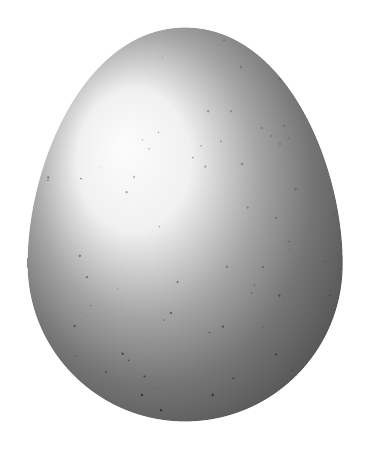
\begin{tikzpicture}
            \colorlet{myEgg}{gray!70!gray!50}
            \draw[looseness=0.9,ball color=white!70!gray!50,draw=none,clip] (-2,0) arc (180:360:2) to[out=90,in=0] (0,3) to[out=180,in=90] (-2,0) -- cycle;
            \foreach \x in {1,...,100}
                {   \pgfmathsetmacro{\rDot}{random()/50}
                    \pgfmathsetmacro{\xCoo}{rand*2}
                    \pgfmathsetmacro{\yCoo}{rand*2.5+0.5}
                    \pgfmathsetmacro{\dColor}{100-60*sqrt(pow(\xCoo+0.5,2)+pow(\yCoo-1.4,2))/2.6}
                    \fill[myEgg!\dColor!black] (\xCoo,\yCoo) circle (\rDot);
                }
        \end{tikzpicture}
        \caption{デザインした象の卵の形状}
        \label{figure:elephants_egg}
    \end{center}
\end{figure}
%------!!

\subsection{大きさ}
\section{デザインプロセス}
数式(\ref{eq:egg_equation})は、山本\cite{Yamamoto}が検討した卵形曲線の方程式のうちの一つである。

\begin{eqnarray}
    \label{eq:egg_equation}
    (x^2 + y^2)^2 = ax^3 + (a - b)xy^2 \ \ \ \ \ (ただし、\ a \ge b \ge 0)
\end{eqnarray}


\section{結果}
論文に掲載した図表は必ず本文で説明すること。
一般的に図のキャプション(タイトル)は下に、表のキャプションは上につけます。
図表については、TeXのコード内で必ず\verb#\label{    }#を編集し、
図表番号も数字を記入せずに\verb#\ref{    }#を用いること。

図\ref{figure:Phoca_groenlandica}にタテゴトアザラシの赤ちゃんの写真を示す。
この通り、愛らしい。
表\ref{table:SpeedOfLightTate}と


% ----- 図:タテゴトアザラシの赤ちゃん ------
\begin{figure}[htbp]
    \begin{center}
        \includegraphics[width=100mm]{hoca_groenlandica.pdf}
        \caption{タテゴトアザラシの赤ちゃん}
        \label{figure:Phoca_groenlandica}
    \end{center}
\end{figure}
% -----ここまで図:タテゴトアザラシの赤ちゃん ------  

% -----表:光速度の測定の歴史 ------
\begin{landscape}%表を90度回転させたい時にこれで囲む
    \begin{table}[!ph]
        \caption{光速度の測定の歴史(縦)}
        \label{table:SpeedOfLightTate}
        \vspace{5mm}
        \centering
        \begin{tabular}{llll}
            \bhline
            病院名  & 取り組み     & コンセプト              & 課題         \\
            \hline
            1638 & Galileo  & 二人が離れてランプの         & (音速10倍以上)  \\
                 &          & 光を見る               &            \\
            1675 & Roemer   & 木星の衛星の観測から         & 2          \\
            1728 & Bradley  & 星の収差から             & 3.01       \\
            1849 & Fizeau   & 高速に回転する歯車を通過する光を見る & 3.133      \\
            1862 & Foucault & 高速に回転する鏡の光の角度変化    & 2.99796    \\
            2022 & Aozora   & 象の卵の疑似孵化実験から       & 2.99792458 \\
            \hline
        \end{tabular}
    \end{table}
\end{landscape}
% -----ここまで表:光速度の測定の歴史 ------

% -----表:光速度の測定の歴史 ------
% \begin{landscape}%表を90度回転させたい時にこれで囲む
% \begin{table}[!ph]
%     \caption{光速度の測定の歴史(横)}
%     \label{table:SpeedOfLightYoko}
%     \vspace{5mm}
%     \centering
%         \begin{tabular}{llll}
%         \bhline
%         病院名 & 取り組み & コンセプト & 課題 \\
%         \hline
%         1638 & Galileo & 二人が離れてランプの & (音速10倍以上) \\
%          &  & 光を見る &  \\           
%         1675 & Roemer & 木星の衛星の観測から & 2 \\
%         1728 & Bradley & 星の収差から & 3.01 \\
%         1849 & Fizeau & 高速に回転する歯車を通過する光を見る & 3.133 \\
%         1862 & Foucault & 高速に回転する鏡の光の角度変化 & 2.99796 \\
%         2022 & Aozora & 象の卵の疑似孵化実験から & 2.99792458 \\
%         \hline
%          \end{tabular}
% \end{table}
% \end{landscape}
% -----ここまで表:光速度の測定の歴史 ------ 

\chapter{結論}

\pagestyle{fancy}
\fancyhead{} % clear all header fields
\lhead{謝辞} %ヘッダ左
\chead{} %ヘッダ中央
\rhead{\thepage} %ヘッダ右.コンパイルした日付を表示
\lfoot{} %フッタ左
\cfoot{} %フッタ中央.ページ番号を表示
% \rfoot{造形・メディアデザインコース} %フッタ右
\renewcommand{\footrulewidth}{0.5pt} %フッタの罫線


\chapter*{謝辞}
\addcontentsline{toc}{chapter}{謝辞} %謝辞を目次に掲載するための処理
謝辞はお世話になった人へ感謝の意を述べる大事な章です。
先輩の論文のコピペではなく論文作成に協力を頂いた方等への感謝の気持ちを
自分の言葉で簡潔にまとめて書きましょう。
ただし、くだけ過ぎた文章は良くありません。
論文にふさわしい文章となるように気をつけましょう。
対象は、研究指導を担当してもらった先生(指導教員、主査、副査)、
アドバイス等を頂いたそれ以外の先生(研究会などで重要な意見をもらった他大学の先生含む)、
研究協力をして頂いた人たち(先輩、後輩、同期等)です。

\newpage
\pagestyle{fancy}
\fancyhead{} % clear all header fields
\lhead{参考文献} %ヘッダ左
% \renewcommand{\chaptermark}[1]{\lhead{第\ \thechapter\ 章~~~#1}{}}
\chead{} %ヘッダ中央
\rhead{\thepage} %ヘッダ右.コンパイルした日付を表示
\lfoot{} %フッタ左
\cfoot{} %フッタ中央.ページ番号を表示
% \rfoot{造形・メディアデザインコース} %フッタ右
\renewcommand{\footrulewidth}{0.5pt} %フッタの罫線

%------参考文献    
\pagestyle{fancy}
\fancyhead{} % clear all header fields
\lhead{参考文献} %ヘッダ左
\renewcommand{\chaptermark}[1]{\lhead{参考文献\ \thechapter\ ~~~#1}{}}
\chead{} %ヘッダ中央
\rhead{\thepage} %ヘッダ右.コンパイルした日付を表示
\lfoot{} %フッタ左
\cfoot{} %フッタ中央.ページ番号を表示
% \rfoot{造形・メディアデザインコース} %フッタ右
\renewcommand{\footrulewidth}{0.5pt} %フッタの罫線
\titleformat{\chapter}[display]{\huge\bfseries}{参考文献\ \thechapter}{20pt}{}[]

\begin{thebibliography}{99} % 参考文献

    \bibitem{Web1} % 論文
    %  著者: 論文タイトル, 掲載論文誌名, 掲載号, 掲載年.
    ICT総研: 2022年度SNS利用動向に関する調査,
    \url{https://ictr.co.jp/report/20220517-2.html/}(参照 2024).

    \bibitem{Thesis1} % 本
    %  著者: 翻訳本のタイトル, 出版社, ページ数, 発行年.
    森本洋一.メッセージングアプリの機能がコミュニケーションにおいて果たす役割に関する一考察,
    専修大学情報科学研究所所報, 86, pp19-24, 2016.

    \bibitem{Thesis2}
    岡本卓也: SNSストレス尺度の作成とSNS利用動機の違いによるSNSストレス,
    信州大学人文科学論集, 4, pp113-131, 2017.

    \bibitem{Thesis3}
    小澤 賢司, 清水 忍: フェイスマークが伝える感性情報,

    \bibitem{Thesis4}
    野村竜成,田村良一: メッセージングアプリケーションにおける感情伝達のための表現方法に関する研究,
    日本感性工学論文誌, 21(3), pp309-316, 2022.

    \bibitem{Thesis5}
    Toshiki Aoki, Rintaro Chujo, Katsufumi Matsui, Saemi Choi, Ari Hautasaari:
    EmoBalloon - Conveying Emotional Arousal in Text Chats with Speech Balloons,
    In CHI Conference on Human Factors in Computing Systems, (CHI '22), Article 527, 1–16, 2022.

    \bibitem{book1} % 本
    %  著者: 翻訳本のタイトル, 出版社, ページ数, 発行年.

    \bibitem{Book2} % 翻訳本
    %  著者, 翻訳者(訳): 翻訳本のタイトル, 出版社, ページ数, 発行年.
    ジョゼ・サラマーゴ, 木下 眞穂(訳): 象の旅, 書肆侃侃房, 216p, 2021.

    \bibitem{Web} % Webサイト
    %  サイト名:ページ名(オンライン),\url{https://} (参照 2021-12-34).
    香川大学:造形・メディアデザインコース(オンライン), \url{https://www.kagawa-u.ac.jp/kagawa-u_ead/course/modeling/} (参照 2021-12-24).

    \bibitem{Yamamoto} % Webサイト
    %  サイト名:ページ名(オンライン),\url{https://} (参照 2021-12-34).
    TDCC LABORATORY:卵形曲線を表す方程式(オンライン), \url{https://nyjp07.com/index_egg.html} (参照 2021-1-10).

\end{thebibliography}
%------ここまで参考文献

%------付録
\newpage
\appendix         % 付録
\pagestyle{fancy}
\fancyhead{} % clear all header fields
% \lhead{付録} %ヘッダ左
\renewcommand{\chaptermark}[1]{\lhead{付録\ \thechapter\ ~~~#1}{}}
\chead{} %ヘッダ中央
\rhead{\thepage} %ヘッダ右.コンパイルした日付を表示
\lfoot{} %フッタ左
\cfoot{} %フッタ中央.ページ番号を表示
% \rfoot{造形・メディアデザインコース} %フッタ右
\renewcommand{\footrulewidth}{0.5pt} %フッタの罫線
\titleformat{\chapter}[display]{\huge\bfseries}{付録\ \thechapter}{20pt}{}[]

\chapter{インターネットアンケート画面}
\section{象の卵に関するインターネットアンケート画面}
\section{デザインした象の卵のインターネット評価アンケート画面}

\titleformat{\chapter}[display]{\huge\bfseries}{付録\ \thechapter}{20pt}{}[]

\chapter{インターネットアンケート画面}
\section{象の卵に関するインターネットアンケート画面}
\section{デザインした象の卵のインターネット評価アンケート画面}

%------ここまで付録

\end{document}
